\documentclass{article}
\usepackage{fancyhdr}
\usepackage{extramarks}
\usepackage{amsmath}
\usepackage{amsthm}
\usepackage{amsfonts}
\usepackage{tikz}
\usepackage[plain]{algorithm}
\usepackage{algpseudocode}
\usepackage{multirow}
\usepackage{circuitikz}
\usepackage{amssymb}
\usepackage{booktabs}
\usetikzlibrary{automata,positioning,shapes.geometric, arrows.meta, calc}

% Custom Commands
\newcommand{\xmark}{%
\tikz[scale=0.23] {
    \draw[line width=0.7,line cap=round] (0,0) to [bend left=6] (1,1);
    \draw[line width=0.7,line cap=round] (0.2,0.95) to [bend right=3] (0.8,0.05);
}}
\newcommand{\cmark}{%
\tikz[scale=0.23] {
    \draw[line width=0.7,line cap=round] (0.25,0) to [bend left=10] (1,1);
    \draw[line width=0.8,line cap=round] (0,0.35) to [bend right=1] (0.23,0);
}}

% TikZ Styles
\tikzset{
    bus/.style={draw, thick, minimum width=2.5cm, minimum height=0.2cm}, 
    generator/.style={circle, draw, thick, minimum size=0.8cm, path picture={
        \draw (path picture bounding box.south west) .. controls ($(path picture bounding box.center)-(0.2cm,0.2cm)$) and ($(path picture bounding box.center)+(0.2cm,0.2cm)$) .. (path picture bounding box.north east);
        \draw (path picture bounding box.north west) .. controls ($(path picture bounding box.center)-(0.2cm,-0.2cm)$) and ($(path picture bounding box.center)+(0.2cm,-0.2cm)$) .. (path picture bounding box.south east);
    }},
    load/.style={regular polygon, regular polygon sides=3, draw, thick, fill=gray!20, minimum size=0.8cm, shape border rotate=180},
    line/.style={thick},
    label style/.style={font=\small, align=center},
    bus label/.style={font=\small, above},
    power_arrow/.style={thick, ->},
    load_connector/.style={line width=3pt, gray!70}
}

\usepackage{graphicx}
\graphicspath{ {./images/} }

%% Basic Document Settings
\topmargin=-0.45in
\evensidemargin=0in
\oddsidemargin=0in
\textwidth=6.5in
\textheight=9.0in
\headsep=0.25in
\linespread{1.1}

\pagestyle{fancy}
\lhead{Yousef Alaa Awad}
\chead{\hmwkClass\: \hmwkTitle}
\rhead{\firstxmark}
\lfoot{\lastxmark}
\cfoot{\thepage}

\renewcommand\headrulewidth{0.4pt}
\renewcommand\footrulewidth{0.4pt}

\setlength\parindent{0pt}

%% Create Problem Sections
\setcounter{secnumdepth}{0}
\newcounter{partCounter}
\newcounter{homeworkProblemCounter}
\setcounter{homeworkProblemCounter}{1}

\newcommand{\hmwkTitle}{Homework\ \#12}
\newcommand{\hmwkClass}{Power Systems Economics}

%% Title Page
\title{
    \vspace{2in}
    \textmd{\textbf{\hmwkClass:\ \hmwkTitle}}\\
    \normalsize\vspace{0.1in}
    \vspace{3in}
}

\author{Yousef Alaa Awad}

% Problems start here
\begin{document}

\maketitle
\pagebreak

\section{6.10}
\textbf{Given:} \textit{Consider the two-bus power system of Problem 6.2. Given that $K = R/V^2 = 0.0001 \text{ MW}^{-1}$ for the line connecting buses A and B. Calculate the value of the flow that minimizes the total variable cost of production.}

\begin{center}
  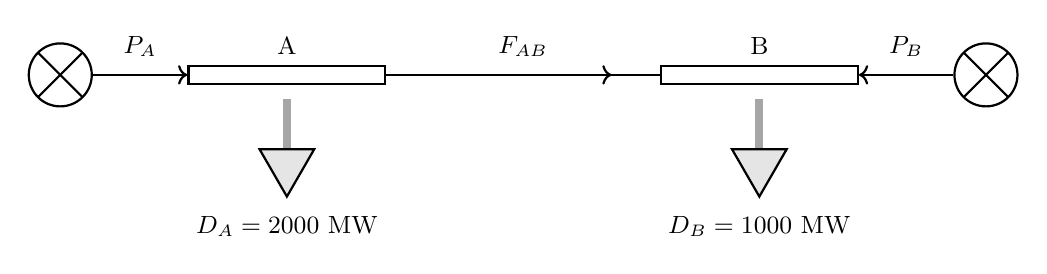
\begin{tikzpicture}
      % --- Nodes for Buses ---
      \node (busA) [bus] at (0,0) {};
      \node[bus label] at (busA.north) {A};
      \node (busB) [bus] at (6,0) {};
      \node[bus label] at (busB.north) {B};

      % --- Generators ---
      \node (genA) [generator, left=1.2cm of busA.west] {};
      \node (genB) [generator, right=1.2cm of busB.east] {};
      \draw[power_arrow] (genA.east) -- (busA.west) node[above=0.1cm, midway, font=\small] {$P_A$};
      \draw[power_arrow] (genB.west) -- (busB.east) node[above=0.1cm, midway, font=\small] {$P_B$}; 

      % --- Loads ---
      \node (loadA_shape) [load, below=0.8cm of busA.south] {};
      \draw[load_connector] ($(busA.south) - (0,0.5em)$) -- (loadA_shape.north);
      \node[below=0.1cm of loadA_shape.south, font=\small] {$D_A = 2000 \text{ MW}$};

      \node (loadB_shape) [load, below=0.8cm of busB.south] {};
      \draw[load_connector] ($(busB.south) - (0,0.5em)$) -- (loadB_shape.north);
      \node[below=0.1cm of loadB_shape.south, font=\small] {$D_B = 1000 \text{ MW}$};

      % --- Transmission Line ---
      \draw[line] (busA.east) -- (busB.west);
      \node (fab_label) at ($ (busA.east)!0.5!(busB.west) $) {}; 
      \draw[power_arrow] ($(fab_label.west)-(1cm,0)$) -- ($(fab_label.east)+(1cm,0)$)
          node[above=0.1cm, midway, font=\small] {$F_{AB}$};
  \end{tikzpicture}
\end{center}

First, we define the problem mathematically. We want to minimize the total cost $C_{Total} = C_A(P_A) + C_B(P_B)$.
The marginal cost functions are:
$$ MC_A = 20 + 0.03 P_A $$
$$ MC_B = 15 + 0.02 P_B $$

We define $F$ as the power flow received at Bus A from Bus B. Since Generator B is cheaper ($15\$$ base vs $20\$$), power will flow from B to A.
At Bus A, the load is met by local generation plus the received flow:
$$ P_A + F = D_A \implies P_A = 2000 - F $$

At Bus B, the generation must supply the local load, plus the flow sent to A, plus the transmission losses.
$$ P_B = D_B + F + P_{Loss} $$
We are given $P_{Loss} = K \cdot F^2 = 0.0001 F^2$.
$$ P_B = 1000 + F + 0.0001 F^2 $$

To find the minimum cost, we look for the point where the marginal benefit of importing one more MW at Bus A equals the marginal cost of producing and sending it from Bus B.
Mathematically, this is the chain rule derivative of the cost function with respect to flow $F$:
$$ \frac{dC}{dF} = \frac{dC_A}{dP_A}\frac{dP_A}{dF} + \frac{dC_B}{dP_B}\frac{dP_B}{dF} = 0 $$

Substituting our derivatives:
1. From $P_A = 2000 - F$, we get $\frac{dP_A}{dF} = -1$.
2. From $P_B = 1000 + F + 0.0001 F^2$, we get $\frac{dP_B}{dF} = 1 + 0.0002 F$.

Substituting these into the optimality condition:
$$ MC_A \cdot (-1) + MC_B \cdot (1 + 0.0002 F) = 0 $$
$$ MC_A = MC_B (1 + 0.0002 F) $$
This equation tells us that at the optimal point, the price at A must equal the price at B scaled by the penalty factor due to incremental losses.

Now, we solve for $F$. Let's test the value $F = 730$ MW to see if it satisfies this condition.
\begin{itemize}
    \item \textbf{Calculate $P_A$:} $P_A = 2000 - 730 = 1270$ MW.
    \item \textbf{Calculate $MC_A$:} $MC_A = 20 + 0.03(1270) = 20 + 38.1 = 58.10$ \$/MWh.
    \item \textbf{Calculate $P_B$:} $P_B = 1000 + 730 + 0.0001(730^2) = 1730 + 53.29 = 1783.29$ MW.
    \item \textbf{Calculate $MC_B$:} $MC_B = 15 + 0.02(1783.29) = 15 + 35.666 = 50.666$ \$/MWh.
    \item \textbf{Check Optimality:}
    $$ \text{RHS} = MC_B(1 + 0.0002 \times 730) = 50.666(1 + 0.146) = 50.666(1.146) $$
    $$ \text{RHS} = 58.06 \approx 58.10 $$
\end{itemize}
The values match very closely (within rounding error). Therefore, the optimal flow is indeed \textbf{730 MW}.

\bigskip
\textbf{Results:}
\begin{itemize}
    \item Flow $F_{BA} = 730$ MW.
    \item Generation $P_A = 1270$ MW.
    \item Generation $P_B = 1783$ MW.
    \item Losses = 53 MW.
    \item Nodal Price $\pi_A = MC_A = \$58.10$/MWh.
    \item Nodal Price $\pi_B = MC_B = \$50.67$/MWh.
\end{itemize}

\textbf{Merchandising Surplus Calculation:}
$$ \text{Consumer Pay} = (2000 \times 58.10) + (1000 \times 50.67) = 116,200 + 50,670 = \$166,870 $$
$$ \text{Gen Revenue} = (1270 \times 58.10) + (1783 \times 50.67) = 73,787 + 90,344.61 = \$164,131.61 $$
$$ \text{Surplus} = 166,870 - 164,131.61 = \$2,738.39 $$

\pagebreak

\section{6.15}
\textbf{Given:} \textit{Show that purchasing 100 MW of point-to-point financial rights between buses 3 and 1 provides a perfect hedge to Generator D.}

First, we recall the nodal prices from Problem 6.8: $\pi_1 = \$13.33$ (Consumer) and $\pi_3 = \$10.00$ (Generator). Generator D wants to sell 100 MW at a strike price of $K = \$11.00$.

We analyze the cash flows:

\textbf{1. Market Revenue:}
Generator D sells 100 MW at its local price $\pi_3$.
$$ \text{Rev}_{Mkt} = 100 \times 10.00 = +\$1000 $$

\textbf{2. CfD Payment:}
Generator pays the difference between the sink price $\pi_1$ and the strike price $K$.
$$ \text{Pay}_{CfD} = 100 \times (\pi_1 - K) = 100 \times (13.33 - 11.00) = 100 \times 2.33 = -\$233 $$

\textbf{3. FTR Payout:}
The FTR pays the difference between sink and source prices.
$$ \text{Pay}_{FTR} = 100 \times (\pi_1 - \pi_3) = 100 \times (13.33 - 10.00) = 100 \times 3.33 = +\$333 $$

\textbf{Total Net Revenue:}
$$ \text{Total} = 1000 - 233 + 333 = \$1100 $$

\textbf{Target:}
$$ 100 \text{ MW} \times \$11.00 = \$1100 $$

Since Total Revenue equals Target Revenue, the hedge is perfect.

\end{document}
